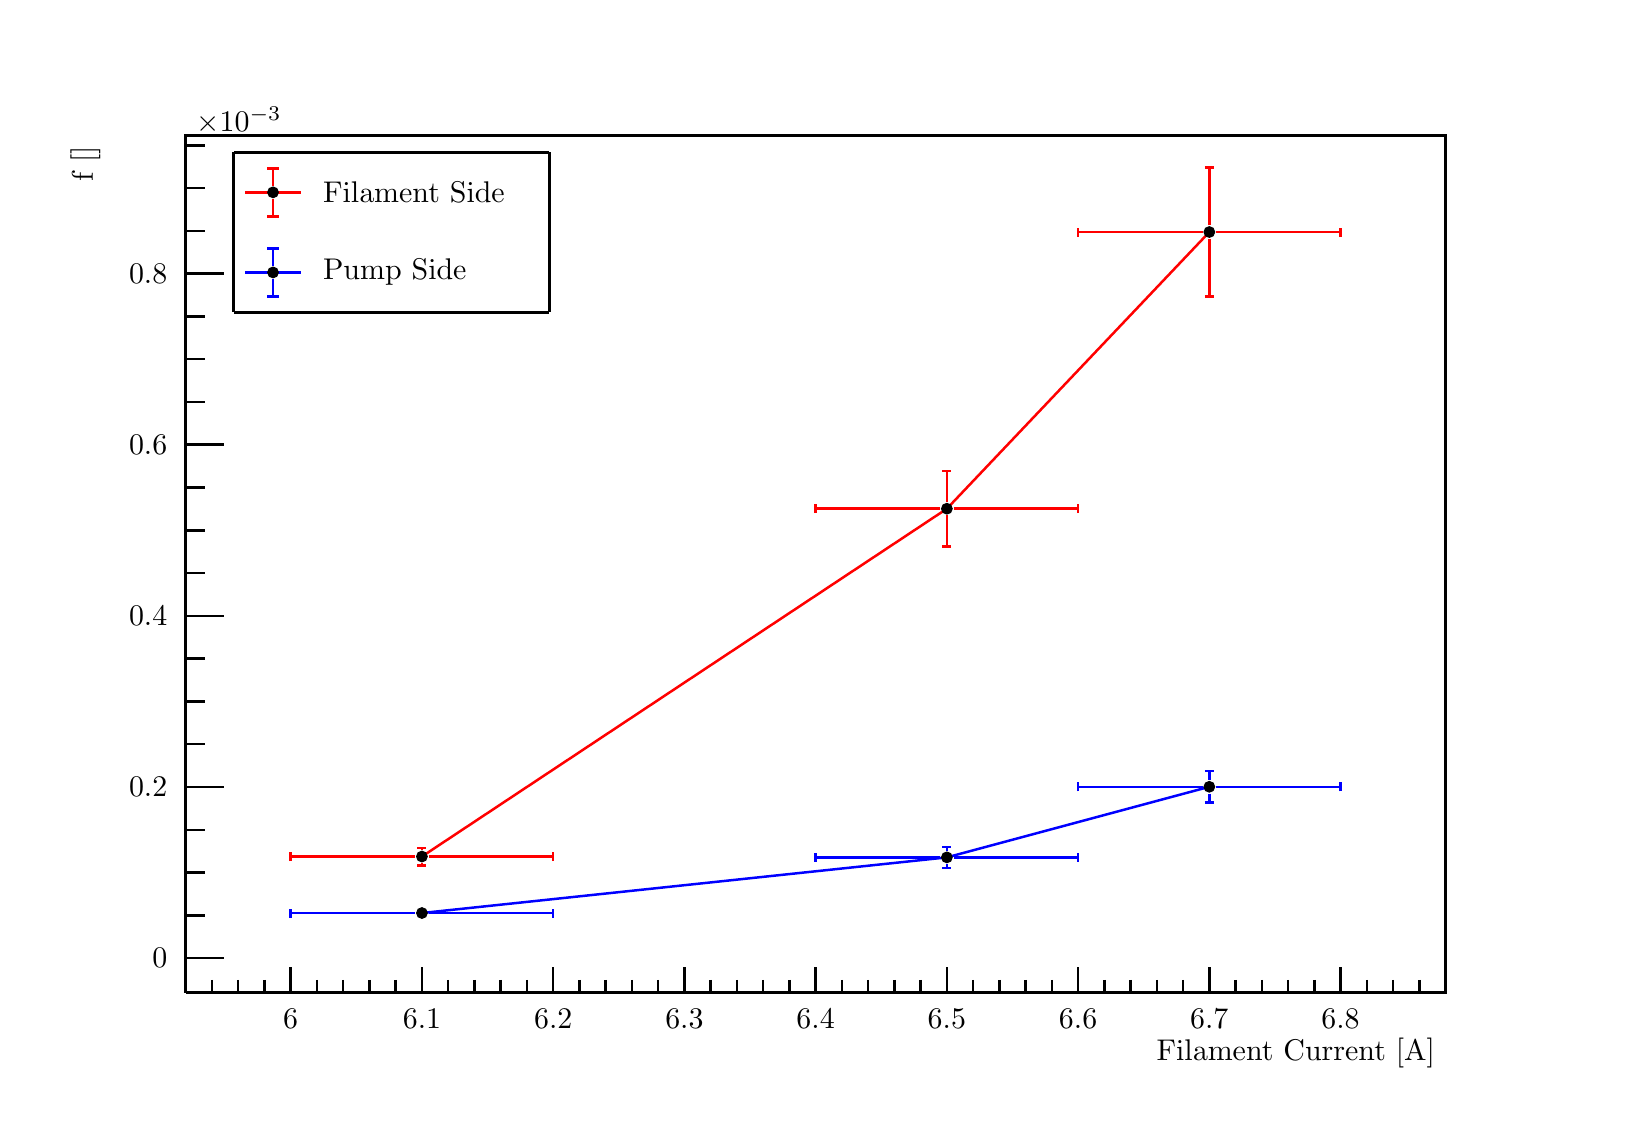
\begin{tikzpicture}
\pgfdeclareplotmark{cross} {
\pgfpathmoveto{\pgfpoint{-0.3\pgfplotmarksize}{\pgfplotmarksize}}
\pgfpathlineto{\pgfpoint{+0.3\pgfplotmarksize}{\pgfplotmarksize}}
\pgfpathlineto{\pgfpoint{+0.3\pgfplotmarksize}{0.3\pgfplotmarksize}}
\pgfpathlineto{\pgfpoint{+1\pgfplotmarksize}{0.3\pgfplotmarksize}}
\pgfpathlineto{\pgfpoint{+1\pgfplotmarksize}{-0.3\pgfplotmarksize}}
\pgfpathlineto{\pgfpoint{+0.3\pgfplotmarksize}{-0.3\pgfplotmarksize}}
\pgfpathlineto{\pgfpoint{+0.3\pgfplotmarksize}{-1.\pgfplotmarksize}}
\pgfpathlineto{\pgfpoint{-0.3\pgfplotmarksize}{-1.\pgfplotmarksize}}
\pgfpathlineto{\pgfpoint{-0.3\pgfplotmarksize}{-0.3\pgfplotmarksize}}
\pgfpathlineto{\pgfpoint{-1.\pgfplotmarksize}{-0.3\pgfplotmarksize}}
\pgfpathlineto{\pgfpoint{-1.\pgfplotmarksize}{0.3\pgfplotmarksize}}
\pgfpathlineto{\pgfpoint{-0.3\pgfplotmarksize}{0.3\pgfplotmarksize}}
\pgfpathclose
\pgfusepathqstroke
}
\pgfdeclareplotmark{cross*} {
\pgfpathmoveto{\pgfpoint{-0.3\pgfplotmarksize}{\pgfplotmarksize}}
\pgfpathlineto{\pgfpoint{+0.3\pgfplotmarksize}{\pgfplotmarksize}}
\pgfpathlineto{\pgfpoint{+0.3\pgfplotmarksize}{0.3\pgfplotmarksize}}
\pgfpathlineto{\pgfpoint{+1\pgfplotmarksize}{0.3\pgfplotmarksize}}
\pgfpathlineto{\pgfpoint{+1\pgfplotmarksize}{-0.3\pgfplotmarksize}}
\pgfpathlineto{\pgfpoint{+0.3\pgfplotmarksize}{-0.3\pgfplotmarksize}}
\pgfpathlineto{\pgfpoint{+0.3\pgfplotmarksize}{-1.\pgfplotmarksize}}
\pgfpathlineto{\pgfpoint{-0.3\pgfplotmarksize}{-1.\pgfplotmarksize}}
\pgfpathlineto{\pgfpoint{-0.3\pgfplotmarksize}{-0.3\pgfplotmarksize}}
\pgfpathlineto{\pgfpoint{-1.\pgfplotmarksize}{-0.3\pgfplotmarksize}}
\pgfpathlineto{\pgfpoint{-1.\pgfplotmarksize}{0.3\pgfplotmarksize}}
\pgfpathlineto{\pgfpoint{-0.3\pgfplotmarksize}{0.3\pgfplotmarksize}}
\pgfpathclose
\pgfusepathqfillstroke
}
\pgfdeclareplotmark{newstar} {
\pgfpathmoveto{\pgfqpoint{0pt}{\pgfplotmarksize}}
\pgfpathlineto{\pgfqpointpolar{44}{0.5\pgfplotmarksize}}
\pgfpathlineto{\pgfqpointpolar{18}{\pgfplotmarksize}}
\pgfpathlineto{\pgfqpointpolar{-20}{0.5\pgfplotmarksize}}
\pgfpathlineto{\pgfqpointpolar{-54}{\pgfplotmarksize}}
\pgfpathlineto{\pgfqpointpolar{-90}{0.5\pgfplotmarksize}}
\pgfpathlineto{\pgfqpointpolar{234}{\pgfplotmarksize}}
\pgfpathlineto{\pgfqpointpolar{198}{0.5\pgfplotmarksize}}
\pgfpathlineto{\pgfqpointpolar{162}{\pgfplotmarksize}}
\pgfpathlineto{\pgfqpointpolar{134}{0.5\pgfplotmarksize}}
\pgfpathclose
\pgfusepathqstroke
}
\pgfdeclareplotmark{newstar*} {
\pgfpathmoveto{\pgfqpoint{0pt}{\pgfplotmarksize}}
\pgfpathlineto{\pgfqpointpolar{44}{0.5\pgfplotmarksize}}
\pgfpathlineto{\pgfqpointpolar{18}{\pgfplotmarksize}}
\pgfpathlineto{\pgfqpointpolar{-20}{0.5\pgfplotmarksize}}
\pgfpathlineto{\pgfqpointpolar{-54}{\pgfplotmarksize}}
\pgfpathlineto{\pgfqpointpolar{-90}{0.5\pgfplotmarksize}}
\pgfpathlineto{\pgfqpointpolar{234}{\pgfplotmarksize}}
\pgfpathlineto{\pgfqpointpolar{198}{0.5\pgfplotmarksize}}
\pgfpathlineto{\pgfqpointpolar{162}{\pgfplotmarksize}}
\pgfpathlineto{\pgfqpointpolar{134}{0.5\pgfplotmarksize}}
\pgfpathclose
\pgfusepathqfillstroke
}
\definecolor{c}{rgb}{1,1,1};
\draw [color=c, fill=c] (0,0) rectangle (20,13.6103);
\draw [color=c, fill=c] (2,1.36103) rectangle (18,12.2493);
\definecolor{c}{rgb}{0,0,0};
\draw [c,line width=0.9] (2,1.36103) -- (2,12.2493) -- (18,12.2493) -- (18,1.36103) -- (2,1.36103);
\definecolor{c}{rgb}{1,1,1};
\draw [color=c, fill=c] (2,1.36103) rectangle (18,12.2493);
\definecolor{c}{rgb}{0,0,0};
\draw [c,line width=0.9] (2,1.36103) -- (2,12.2493) -- (18,12.2493) -- (18,1.36103) -- (2,1.36103);
\draw [c,line width=0.9] (2,1.36103) -- (18,1.36103);
\draw [c,line width=0.9] (3.33333,1.68768) -- (3.33333,1.36103);
\draw [c,line width=0.9] (3.66667,1.52436) -- (3.66667,1.36103);
\draw [c,line width=0.9] (4,1.52436) -- (4,1.36103);
\draw [c,line width=0.9] (4.33333,1.52436) -- (4.33333,1.36103);
\draw [c,line width=0.9] (4.66667,1.52436) -- (4.66667,1.36103);
\draw [c,line width=0.9] (5,1.68768) -- (5,1.36103);
\draw [c,line width=0.9] (5.33333,1.52436) -- (5.33333,1.36103);
\draw [c,line width=0.9] (5.66667,1.52436) -- (5.66667,1.36103);
\draw [c,line width=0.9] (6,1.52436) -- (6,1.36103);
\draw [c,line width=0.9] (6.33333,1.52436) -- (6.33333,1.36103);
\draw [c,line width=0.9] (6.66667,1.68768) -- (6.66667,1.36103);
\draw [c,line width=0.9] (7,1.52436) -- (7,1.36103);
\draw [c,line width=0.9] (7.33333,1.52436) -- (7.33333,1.36103);
\draw [c,line width=0.9] (7.66667,1.52436) -- (7.66667,1.36103);
\draw [c,line width=0.9] (8,1.52436) -- (8,1.36103);
\draw [c,line width=0.9] (8.33333,1.68768) -- (8.33333,1.36103);
\draw [c,line width=0.9] (8.66667,1.52436) -- (8.66667,1.36103);
\draw [c,line width=0.9] (9,1.52436) -- (9,1.36103);
\draw [c,line width=0.9] (9.33333,1.52436) -- (9.33333,1.36103);
\draw [c,line width=0.9] (9.66667,1.52436) -- (9.66667,1.36103);
\draw [c,line width=0.9] (10,1.68768) -- (10,1.36103);
\draw [c,line width=0.9] (10.3333,1.52436) -- (10.3333,1.36103);
\draw [c,line width=0.9] (10.6667,1.52436) -- (10.6667,1.36103);
\draw [c,line width=0.9] (11,1.52436) -- (11,1.36103);
\draw [c,line width=0.9] (11.3333,1.52436) -- (11.3333,1.36103);
\draw [c,line width=0.9] (11.6667,1.68768) -- (11.6667,1.36103);
\draw [c,line width=0.9] (12,1.52436) -- (12,1.36103);
\draw [c,line width=0.9] (12.3333,1.52436) -- (12.3333,1.36103);
\draw [c,line width=0.9] (12.6667,1.52436) -- (12.6667,1.36103);
\draw [c,line width=0.9] (13,1.52436) -- (13,1.36103);
\draw [c,line width=0.9] (13.3333,1.68768) -- (13.3333,1.36103);
\draw [c,line width=0.9] (13.6667,1.52436) -- (13.6667,1.36103);
\draw [c,line width=0.9] (14,1.52436) -- (14,1.36103);
\draw [c,line width=0.9] (14.3333,1.52436) -- (14.3333,1.36103);
\draw [c,line width=0.9] (14.6667,1.52436) -- (14.6667,1.36103);
\draw [c,line width=0.9] (15,1.68768) -- (15,1.36103);
\draw [c,line width=0.9] (15.3333,1.52436) -- (15.3333,1.36103);
\draw [c,line width=0.9] (15.6667,1.52436) -- (15.6667,1.36103);
\draw [c,line width=0.9] (16,1.52436) -- (16,1.36103);
\draw [c,line width=0.9] (16.3333,1.52436) -- (16.3333,1.36103);
\draw [c,line width=0.9] (16.6667,1.68768) -- (16.6667,1.36103);
\draw [c,line width=0.9] (3.33333,1.68768) -- (3.33333,1.36103);
\draw [c,line width=0.9] (3,1.52436) -- (3,1.36103);
\draw [c,line width=0.9] (2.66667,1.52436) -- (2.66667,1.36103);
\draw [c,line width=0.9] (2.33333,1.52436) -- (2.33333,1.36103);
\draw [c,line width=0.9] (2,1.52436) -- (2,1.36103);
\draw [c,line width=0.9] (16.6667,1.68768) -- (16.6667,1.36103);
\draw [c,line width=0.9] (17,1.52436) -- (17,1.36103);
\draw [c,line width=0.9] (17.3333,1.52436) -- (17.3333,1.36103);
\draw [c,line width=0.9] (17.6667,1.52436) -- (17.6667,1.36103);
\draw [anchor=base] (3.33333,0.911891) node[scale=1.08185, color=c, rotate=0]{6};
\draw [anchor=base] (5,0.911891) node[scale=1.08185, color=c, rotate=0]{6.1};
\draw [anchor=base] (6.66667,0.911891) node[scale=1.08185, color=c, rotate=0]{6.2};
\draw [anchor=base] (8.33333,0.911891) node[scale=1.08185, color=c, rotate=0]{6.3};
\draw [anchor=base] (10,0.911891) node[scale=1.08185, color=c, rotate=0]{6.4};
\draw [anchor=base] (11.6667,0.911891) node[scale=1.08185, color=c, rotate=0]{6.5};
\draw [anchor=base] (13.3333,0.911891) node[scale=1.08185, color=c, rotate=0]{6.6};
\draw [anchor=base] (15,0.911891) node[scale=1.08185, color=c, rotate=0]{6.7};
\draw [anchor=base] (16.6667,0.911891) node[scale=1.08185, color=c, rotate=0]{6.8};
\draw [anchor= east] (18,0.598854) node[scale=1.08185, color=c, rotate=0]{Filament Current [A]};
\draw [c,line width=0.9] (2,1.36103) -- (2,12.2493);
\draw [c,line width=0.9] (2.48,1.80081) -- (2,1.80081);
\draw [c,line width=0.9] (2.24,2.34412) -- (2,2.34412);
\draw [c,line width=0.9] (2.24,2.88744) -- (2,2.88744);
\draw [c,line width=0.9] (2.24,3.43075) -- (2,3.43075);
\draw [c,line width=0.9] (2.48,3.97407) -- (2,3.97407);
\draw [c,line width=0.9] (2.24,4.51738) -- (2,4.51738);
\draw [c,line width=0.9] (2.24,5.0607) -- (2,5.0607);
\draw [c,line width=0.9] (2.24,5.60401) -- (2,5.60401);
\draw [c,line width=0.9] (2.48,6.14733) -- (2,6.14733);
\draw [c,line width=0.9] (2.24,6.69064) -- (2,6.69064);
\draw [c,line width=0.9] (2.24,7.23396) -- (2,7.23396);
\draw [c,line width=0.9] (2.24,7.77727) -- (2,7.77727);
\draw [c,line width=0.9] (2.48,8.32059) -- (2,8.32059);
\draw [c,line width=0.9] (2.24,8.8639) -- (2,8.8639);
\draw [c,line width=0.9] (2.24,9.40722) -- (2,9.40722);
\draw [c,line width=0.9] (2.24,9.95053) -- (2,9.95053);
\draw [c,line width=0.9] (2.48,10.4938) -- (2,10.4938);
\draw [c,line width=0.9] (2.48,1.80081) -- (2,1.80081);
\draw [c,line width=0.9] (2.48,10.4938) -- (2,10.4938);
\draw [c,line width=0.9] (2.24,11.0372) -- (2,11.0372);
\draw [c,line width=0.9] (2.24,11.5805) -- (2,11.5805);
\draw [c,line width=0.9] (2.24,12.1238) -- (2,12.1238);
\draw [anchor= east] (1.9,1.80081) node[scale=1.08185, color=c, rotate=0]{0};
\draw [anchor= east] (1.9,3.97407) node[scale=1.08185, color=c, rotate=0]{0.2};
\draw [anchor= east] (1.9,6.14733) node[scale=1.08185, color=c, rotate=0]{0.4};
\draw [anchor= east] (1.9,8.32059) node[scale=1.08185, color=c, rotate=0]{0.6};
\draw [anchor= east] (1.9,10.4938) node[scale=1.08185, color=c, rotate=0]{0.8};
\draw [anchor=base west] (2,12.2969) node[scale=1.08185, color=c, rotate=0]{$\times10^{-3}$};
\draw [anchor= east] (0.726934,12.2493) node[scale=1.08185, color=c, rotate=90]{f []};
\definecolor{c}{rgb}{1,0,0};
\draw [c,line width=0.9] (5,3.09086) -- (11.6667,7.50805) -- (15,11.022);
\definecolor{c}{rgb}{0,0,0};
\foreach \P in {(5,3.09086), (11.6667,7.50805), (15,11.022)}{\draw[mark options={color=c,fill=c},mark size=1.921922pt,mark=*] plot coordinates {\P};}
\definecolor{c}{rgb}{1,0,0};
\draw [c,line width=0.9] (4.91404,3.09086) -- (3.33333,3.09086);
\draw [c,line width=0.9] (3.33333,3.03355) -- (3.33333,3.14817);
\draw [c,line width=0.9] (5.08596,3.09086) -- (6.66667,3.09086);
\draw [c,line width=0.9] (6.66667,3.03355) -- (6.66667,3.14817);
\draw [c,line width=0.9] (5,3.17682) -- (5,3.20223);
\draw [c,line width=0.9] (4.94269,3.20223) -- (5.05731,3.20223);
\draw [c,line width=0.9] (5,3.0049) -- (5,2.97949);
\draw [c,line width=0.9] (4.94269,2.97949) -- (5.05731,2.97949);
\draw [c,line width=0.9] (11.5807,7.50805) -- (10,7.50805);
\draw [c,line width=0.9] (10,7.45074) -- (10,7.56535);
\draw [c,line width=0.9] (11.7526,7.50805) -- (13.3333,7.50805);
\draw [c,line width=0.9] (13.3333,7.45074) -- (13.3333,7.56535);
\draw [c,line width=0.9] (11.6667,7.59401) -- (11.6667,7.98868);
\draw [c,line width=0.9] (11.6094,7.98868) -- (11.724,7.98868);
\draw [c,line width=0.9] (11.6667,7.42209) -- (11.6667,7.02741);
\draw [c,line width=0.9] (11.6094,7.02741) -- (11.724,7.02741);
\draw [c,line width=0.9] (14.914,11.022) -- (13.3333,11.022);
\draw [c,line width=0.9] (13.3333,10.9646) -- (13.3333,11.0793);
\draw [c,line width=0.9] (15.086,11.022) -- (16.6667,11.022);
\draw [c,line width=0.9] (16.6667,10.9646) -- (16.6667,11.0793);
\draw [c,line width=0.9] (15,11.1079) -- (15,11.8407);
\draw [c,line width=0.9] (14.9427,11.8407) -- (15.0573,11.8407);
\draw [c,line width=0.9] (15,10.936) -- (15,10.2032);
\draw [c,line width=0.9] (14.9427,10.2032) -- (15.0573,10.2032);
\definecolor{c}{rgb}{0,0,1};
\draw [c,line width=0.9] (4.91404,2.37334) -- (3.33333,2.37334);
\draw [c,line width=0.9] (3.33333,2.31604) -- (3.33333,2.43065);
\draw [c,line width=0.9] (5.08596,2.37334) -- (6.66667,2.37334);
\draw [c,line width=0.9] (6.66667,2.31604) -- (6.66667,2.43065);
\draw [c,line width=0.9] (11.5807,3.08006) -- (10,3.08006);
\draw [c,line width=0.9] (10,3.02275) -- (10,3.13737);
\draw [c,line width=0.9] (11.7526,3.08006) -- (13.3333,3.08006);
\draw [c,line width=0.9] (13.3333,3.02275) -- (13.3333,3.13737);
\draw [c,line width=0.9] (11.6667,3.16602) -- (11.6667,3.21441);
\draw [c,line width=0.9] (11.6094,3.21441) -- (11.724,3.21441);
\draw [c,line width=0.9] (11.6667,2.9941) -- (11.6667,2.9457);
\draw [c,line width=0.9] (11.6094,2.9457) -- (11.724,2.9457);
\draw [c,line width=0.9] (14.914,3.97644) -- (13.3333,3.97644);
\draw [c,line width=0.9] (13.3333,3.91913) -- (13.3333,4.03374);
\draw [c,line width=0.9] (15.086,3.97644) -- (16.6667,3.97644);
\draw [c,line width=0.9] (16.6667,3.91913) -- (16.6667,4.03374);
\draw [c,line width=0.9] (15,4.0624) -- (15,4.17688);
\draw [c,line width=0.9] (14.9427,4.17688) -- (15.0573,4.17688);
\draw [c,line width=0.9] (15,3.89048) -- (15,3.77599);
\draw [c,line width=0.9] (14.9427,3.77599) -- (15.0573,3.77599);
\draw [c,line width=0.9] (5,2.37334) -- (11.6667,3.08006) -- (15,3.97644);
\definecolor{c}{rgb}{0,0,0};
\foreach \P in {(5,2.37334), (11.6667,3.08006), (15,3.97644)}{\draw[mark options={color=c,fill=c},mark size=1.921922pt,mark=*] plot coordinates {\P};}
\definecolor{c}{rgb}{1,1,1};
\draw [color=c, fill=c] (2.60745,10) rectangle (6.61891,12.0344);
\definecolor{c}{rgb}{0,0,0};
\draw [c,line width=0.9] (2.60745,10) -- (6.61891,10);
\draw [c,line width=0.9] (6.61891,10) -- (6.61891,12.0344);
\draw [c,line width=0.9] (6.61891,12.0344) -- (2.60745,12.0344);
\draw [c,line width=0.9] (2.60745,12.0344) -- (2.60745,10);
\draw [anchor= west] (3.61032,11.5258) node[scale=1.08185, color=c, rotate=0]{Filament Side};
\definecolor{c}{rgb}{1,0,0};
\draw [c,line width=0.9] (2.75788,11.5258) -- (3.45989,11.5258);
\draw [c,line width=0.9] (3.10888,11.6117) -- (3.10888,11.8309);
\draw [c,line width=0.9] (3.10888,11.4398) -- (3.10888,11.2206);
\draw [c,line width=0.9] (3.03868,11.8309) -- (3.17908,11.8309);
\draw [c,line width=0.9] (3.03868,11.2206) -- (3.17908,11.2206);
\definecolor{c}{rgb}{0,0,0};
\foreach \P in {(3.10888,11.5258)}{\draw[mark options={color=c,fill=c},mark size=1.921922pt,mark=*] plot coordinates {\P};}
\draw [anchor= west] (3.61032,10.5086) node[scale=1.08185, color=c, rotate=0]{Pump Side};
\definecolor{c}{rgb}{0,0,1};
\draw [c,line width=0.9] (2.75788,10.5086) -- (3.45989,10.5086);
\draw [c,line width=0.9] (3.10888,10.5946) -- (3.10888,10.8138);
\draw [c,line width=0.9] (3.10888,10.4226) -- (3.10888,10.2034);
\draw [c,line width=0.9] (3.03868,10.8138) -- (3.17908,10.8138);
\draw [c,line width=0.9] (3.03868,10.2034) -- (3.17908,10.2034);
\definecolor{c}{rgb}{0,0,0};
\foreach \P in {(3.10888,10.5086)}{\draw[mark options={color=c,fill=c},mark size=1.921922pt,mark=*] plot coordinates {\P};}
\end{tikzpicture}
